\section{PIR}

首先,我们引用FOCS\cite{FOCS:CGKS95}给出的PIR的明确定义。

\begin{definition}[PIR]
    一个\textit{PIR}协议$\Pi$允许客户端从数据库$\db$中检索记录$\db_\dbidx$,而不向$\servercount$个服务器中任何一个泄露索引$\dbidx$。该协议由算法元组$\Pi = (Setup, Query, Answer, Reconstruct)$组成:
    \begin{itemize}
        \item $Setup(1^\lambda,\dbsize) \rightarrow ck$。给定数据库大小$\dbsize$和安全参数$\lambda$,生成公共参数$ck$。
        \item $Query(ck, \dbidx) \rightarrow \query$。给定公共参数$ck$和要查询的索引$\dbidx$,生成查询$\query$。
        \item $Answer(\db, \query) \rightarrow \answer$。给定查询$\query$,生成回答$\answer$。
        \item $Reconstruct(\answer) \rightarrow \db_\dbidx$。给定回答$\answer$,重构出记录$\db_\dbidx$。
    \end{itemize}
    在这一算法中,我们假设$\servercount$个服务器不能共谋。该协议需要满足两个基本性质:\textbf{正确性}和\textbf{隐私性}。
    \begin{itemize}
        \item \textbf{正确性}:对于任意安全参数$\lambda$,对于任意数据库$\db$和索引$\dbidx$,对于任意多项式次数的查询索引序列$\{\dbidx_0,\dbidx_1, \dots\}$。如果$\servercount$个服务器和客户端按照$\Pi$诚实执行,客户端以概率$1-\negl(\lambda)$输出$\{\db_{\dbidx_0},\db_{\dbidx_1}, \dots\}$。
        \item \textbf{隐私性}:对于任意安全参数$\lambda$,对于任意数据库$\db$,对于任意多项式次数的查询索引序列$\{\dbidx_0,\dbidx_1, \dots\}$。如果$\servercount$个服务器和客户端按照$\Pi$诚实执行,$\servercount$个服务器区分$\dbidx$与一随机索引$\dbidx'$的概率小于$\negl(\lambda)$。
    \end{itemize}
    对于正确性和隐私性更形式化的定义将在后文中给出。
\end{definition}

\paragraph{线性复杂度的PIR协议}
如相关工作所述,PIR的属性限制了单次查询的效率。Beimel\cite{C:BeiIshMal00}等人证明,服务器在单次查询中至少需要进行线性时间的运算。这意味着,对于一个大小为$\dbsize$的数据库,服务器至少需要$O(\dbsize)$的时间来处理一个查询。这一结论是PIR的一个基本属性,也是PIR的一个重要局限。尽管目前有许多工作能够将这种复杂度中的常数项降至较小的值,但仍无法改变线性复杂度的基本现实。一旦数据库规模扩大,PIR的效率就会受到严重影响。本研究不涉及线性复杂度的PIR,因此不会进一步详细讨论。

\subsection{亚线性复杂度的PIR协议}
尽管PIR的性质限制了单次查询的效率,但我们仍然可以将多次PIR的均摊复杂度降至亚线性。需要注意的是,亚线性复杂度的PIR包含两个阶段:\textit{离线预处理阶段}和\textit{在线查询阶段}。在预处理阶段,客户端与服务器并不进行真正的请求,仅生成一些用于加速查询的辅助信息,这些信息被称为 $Hint$。在查询阶段,客户端使用 $Hint$ 来加速查询。离线预处理的复杂度往往仍是线性的,而进行在线查询的复杂度则是亚线性的。将预处理的复杂度均摊到一定数量的查询中,我们可以得到亚线性复杂度的PIR。在此,我们给出一个典型的离线-在线PIR定义\cite{EC:CorKog20}。

\begin{definition}[离线-在线PIR]
    一个\textit{离线-在线PIR}协议$\Pi$允许客户端从数据库$\db$中检索记录$\db_\dbidx$,而不向$\servercount$个服务器中任何一个泄露索引$\dbidx$。该协议由算法元组$\Pi = (Setup, Hint,\\ Query, Answer, Reconstruct, Refresh)$组成:

    \noindent \textbf{离线阶段:}
    \begin{itemize}
        \item $Setup(1^\lambda,\dbsize) \rightarrow \query_\hint$。给定数据库大小$\dbsize$和安全参数$\lambda$,生成$Hint$查询$\query_\hint$。
        \item $Hint(\db, \query_\hint) \rightarrow \hint$。给定数据库$\db$和$Hint$查询$\query_\hint$,生成$Hint$ $\hint$。
    \end{itemize}
    \noindent \textbf{在线阶段:}
    \begin{itemize}
        \item $Query(\hint, \dbidx) \rightarrow (\query, \clientstate)$。给定$Hint$ $\hint$和要查询的索引$\dbidx$,生成查询$\query$。注意,查询$\query$可能包含多个子查询。客户端生成并保存一个私有状态$\clientstate$。
        \item $Answer(\db, \query) \rightarrow \answer$。给定查询$\query$,生成回答$\answer$。
        \item $Reconstruct(\clientstate, \hint, \answer) \rightarrow \db_\dbidx$。给定回答$\answer$,使用$Hint$ $\hint$和私有状态$\clientstate$重构出记录$\db_\dbidx$。
        \item $Refresh(\clientstate, \hint, \answer) \rightarrow \hint$。给定回答$\answer$和私有状态$\clientstate$,更新$Hint$ $\hint$。
    \end{itemize}
    在这一算法中,我们仍假设$\servercount$个服务器不能共谋。该协议需要满足相同的两个基本性质:\textbf{正确性}和\textbf{隐私性}。其定义与PIR的定义类似,这里不再赘述。
\end{definition}

\begin{figure}
    \centering
    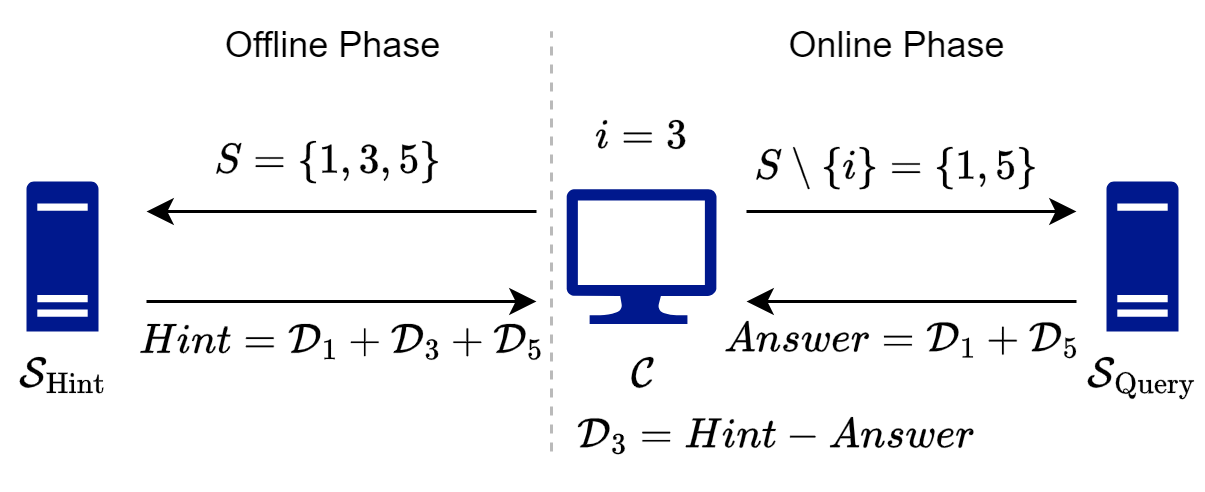
\includegraphics[width=0.5\textwidth]{figure/ck20.png}
    \caption{CK20~\cite{EC:CorKog20} 协议的一个例子。}
    \label{fig:CK20}
\end{figure}

在这些协议中,$Hint$通常由一个包含数据库$\db$中某些索引的集合,以及从这些索引对应的记录中计算出的校验值组成。本文使用"Hint"这个词时,除非特别指明,否则均为兼指集合与校验值。